\subsection{Group versus round-robin tournament}

% Maybe explain the group tournament in more detail
The first experiment we ran was to determine the efficacy of our sampling method. To do this, we compared the win rates of identical decks in a complete round robin tournament (every combination of decks played) with the win rate in a tournament conducted by randomly grouping decks into groups of various sizes, and then playing every combination of the decks within those groups. See for example:

\begin{figure}[t]
	\centering
	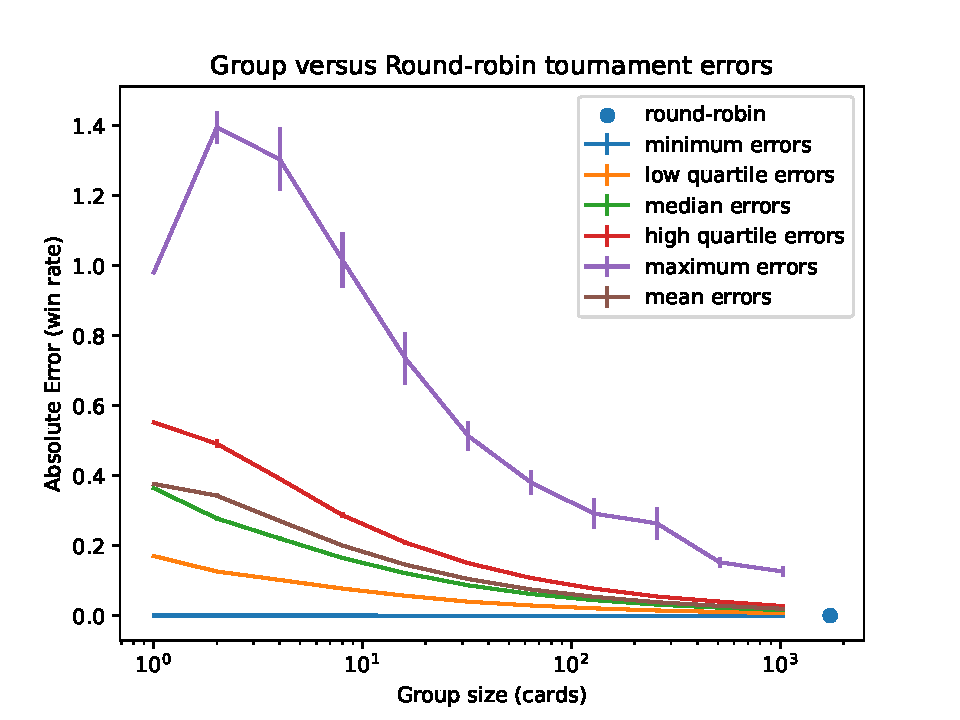
\includegraphics[width=0.9\columnwidth]{group_vs_rr_fig}
	\caption{Absolute value of the difference in win rate between a \textit{group tournament} of varying size and a full round-robin tournamnt of 1728 possible decks, along with error bars}
	\label{fig:group_vs_rr}
\end{figure}

%% Table

We then compute the average error over all of the decks, and we can see a steady convergence of the two values.

% Another table

 \subsection{Optimizing cards without special mechanisms}

The next experiment was to optimize a set of four basic cards, with no extra mechanics. We hypothesized that the `optimal' solution in terms of the standard deviation metric would be to have 4 identical cards, because then there would be only one card and thus zero standard deviation in the winrate of one card. We also recognized, however, that due to the time constraints placed on our optimization algorithm, there was no guarantee it would find this solution. This case seemed even more interesting from a game design perspective, as a game with only a single card is obviously an uninteresting game, so we would like to see what `almost-optimal' solutions appear for this setup. This observation also illustrates a case where the standard deviation metric fails to fully capture the qualities we wish to optimize in our game.

The results of this experiment illustrate a different failure case of our standard deviation metric, one that had not been predicted. The genetic algorithm quickly found this solution: (5/3), (5/4), (8/3), (8/1) which had zero standard deviation. Why? Any pairing of these cards will result in both cards being killed. Thus, every game ends after one round in a tie, and so there is no variance in winrates amongst the decks. 

 \subsection{Optimizing only statistics for special mechanics}

The third experiment was to optimize a number of cards, each with a special mechanic. Each of these cards was assigned an intuitive value for it's attack and health, as a game designer might do. We then optimized over the stats that controlled the special mechanics of these cards. We were interested to see how well it would be possible to optimize the game with these constraints, and how impactful the special mechanics would be for the overall balance of the game. The cards used in this experiment are in Table~\ref{tab:special_cards}.

\begin{table*}[t]
\centering
\begin{tabular}{||c c c c||} 
 \hline
 Card & Attack & Health & Variable Mechanic (see Section~\ref{sec:ab-game-def})\\ [0.5ex] 
 \hline\hline
 Explode On Death & 2 & 1 & Damage dealt to enemies on death \\ 
 \hline
 Friendly Vampire & 1 & 3 & Amount of heath granted to ally \\
 \hline
 Grow On Damage & 0 & 5 & Attack gained per hit taken \\
 \hline
 Heal On Death & 1 & 2 & Health granted to allies on death \\
 \hline
 Health Donor & 1 & 4 & Percent of healing received that is split amongst allies \\
 \hline
 Ignore First Damage & 2 & 1 & Number of attacks which result in no damage taken \\
 \hline
 Morph Attack & 0 & 3 & N/A \\
 \hline
 Pain Splitter & 2 & 2 & Percent of damage taken that is split amongst allies \\
 \hline
 Rampage & 0 & 4 & Middle Age  \\
 \hline
 Survivalist & 2 & 2 & N/A \\
 \hline
 Threshold & 2 & 2 & Number of battles it must survive to damage all opponents on death \\
 \hline
 Time Bomb & 1 & 8 & Number of interactions before it will explode during the next battle \\ 
 \hline
\end{tabular}
\caption{Variable and set parameters for the \textit{optimize special mechanics} experiment}
\label{tab:special_cards}
\end{table*}

The optimizer improved the winrate standard deviation from 0.0751 to 0.0589. 

\subsection{Optimizing health points, attack, and statistics for special mechanics} \label{sec:first_set}

After fixing the attack and health, and focusing solely on the special mechanics, the next logical experiment is to tune both the attack and health, as well as the special mechanics. To reduce the huge dimensionality of this experiment we selected only five cards to optimize. They are listed in Table~\ref{tab:first_set}.

% First Set
\begin{table*}[t]
\centering
\begin{tabular}{||c c c c||} 
 \hline
 Card & Optimized Attack & Optimized Health & Optimized Variable Mechanic (see Section~\ref{sec:ab-game-def})\\ [0.5ex]
 \hline
 Survivalist &  &  & N/A \\
 \hline
 Morph Attack &  &  & N/A \\
 \hline
 Ignore First Damage &  &  & \\
 \hline
 Explode On Death &  &  &  \\ 
 \hline
 Vanilla &  &  &  \\
 \hline
\end{tabular}
\caption{List of cards in the first set, and their optimized solution}
\label{tab:first_set}
\end{table*}

The optimizer improved the winrate standard deviation from 0.0704 to 0.0584. This minimum is approximately the same as the one achieved in the previous experiment, modifying only the values of the special mechanics. 

\subsection{Optimizing after a set rotation}

Another common scenario encountered by designers of trading card games is that of releasing a new set or batch of cards, while maintaining the compatibility, fairness, and competitiveness of the previously released cards. To apply our toolset to this problem we first took the set of five cards and optimized solution found in Section~\ref{sec:first_set}. This represents the first set of cards released. Next we selected another five cards, described in table Table~\ref{tab:second_set}, and optimized them, while keeping the values from the first set fixed at the solution found previously. 

% Compare this to the solution found by treating all 10 cards as one set

% Second Set
\begin{table*}[t]
\centering
\begin{tabular}{||c c c c||} 
 \hline
 Card & Optimized Attack & Optimized Health & Optimized Variable Mechanic (see Section~\ref{sec:ab-game-def})\\ [0.5ex]
 \hline
 Friendly Vampire &  &  &  \\
 \hline
 Grow On Damage &  &  &  \\
 \hline
 Heal On Death &  &  & \\
 \hline
 Rampage &  &  &  \\ 
 \hline
 Vanilla &  &  &  \\
 \hline
\end{tabular}
\caption{List of cards in the second set, and their optimized solution}
\label{tab:second_set}
\end{table*}



% \subsubsection{Optimizing an exhaustive round-robin tournament}
